% プロジェクト学習中間報告書書式テンプレート ver.1.0 (iso-2022-jp)

% 両面印刷する場合は `openany' を削除する
\documentclass[openany,11pt,papersize]{jsbook}
  
  % 報告書提出用スタイルファイル
  \usepackage[final]{funpro}%最終報告書
  %\usepackage[middle]{funpro}%中間報告書

  % 画像ファイル (EPS, EPDF, PNG) を読み込むために
  \usepackage[dvipdfmx]{graphicx,color}
  
  % ファイル分割のためのパッケージ
  \usepackage{subfiles}
  
  % 参考文献管理
\usepackage[
	backend=biber,
	sorting=none,
	style=ieee
]{biblatex}
\addbibresource{ref.bib}

  % ここから -->
  \usepackage{calc,ifthen}
  \newcounter{hoge}
  \newcommand{\fake}[1]{\whiledo{\thehoge<70}{#1\stepcounter{hoge}}%
    \setcounter{hoge}{0}}
  % <-- ここまで 削除してもよい
  
  % 年度の指定
  \thisYear{2017}
  
  % プロジェクト名
  \jProjectName{ビーコンIoTで函館のまちをハックする}
  
  % [簡易版のプロジェクト名]{正式なプロジェクト名}
  % 欧文のプロジェクト名が極端に長い(2行を超える)場合は、短い記述を
  % 任意引数として渡す。
  %\eProjectName[Making Delicious curry]{How to make delicious curry of Hakodate}
  \eProjectName{Leverage the Beacon IoT in Hakodate Real Downtown for Our Smarter Life}
  
  
  % <プロジェクト番号>-<グループ名>
  \ProjectNumber{8-A}
  
  % グループ名
  \jGroupName{Hako-B}
  \eGroupName{Hako-B}
  
  % プロジェクトリーダ
  \ProjectLeader{1015253}{橋場保鷹}{Hodaka~Hashiba}
  
  % グループリーダ
  \GroupLeader  {1015053}{佐藤秀輔}{Shusuke~Sato}
  
  % メンバー数
  \SumOfMembers{4}
  % グループメンバ
  \GroupMember  {1}{1015050}{北原康太}{Kota~Kitahara}
  \GroupMember  {2}{1015053}{佐藤秀輔}{Shusuke~Sato}
  \GroupMember  {3}{1015157}{小笠原瑠奈}{Runa~Ogasawara}
  \GroupMember  {4}{1015204}{小島雄士}{Yuji~Kojima}
  
  % 指導教員
  \jadvisor{松原克弥,藤野雄一,鈴木恵二,奥野拓}
  % 複数人数いる場合はカンマ(,)で区切る。カンマの前後に空白は入れない。
  \eadvisor{Katsuya~Matsubara,Yuichi~Fujino,Keiji~Suzuki,Taku~Okuno}
  
  % 論文提出日
  \jdate{2018年1月19日}
  \edate{January~19, 2018}
  
  \begin{document}
  %
  % 表紙
  \maketitle
  
  %前付け
  \frontmatter
  
  % 和文概要
  \begin{jabstract}
  
  % プロジェクト全体の日本語概要
  \subfile{common/common-jabstract}
  
% プロジェクト全体の日本語概要

本グループは、函館のバスの利用がうまくできていないという問題点に目をつけ函館のバスを快適に利用できるアプリケーションの開発を行うこととした。
問題点を下に、私たちはどのようにビーコンを用いてバス利用を改善していくかを担当の教員の方からレビューを受けながらアイデアを固めた。
そのアイデアなどを下にサービス設計を行い、後期の活動から開発をするための準備を行った。
7月14日に行われた中間発表会ではビーコンの特性を活かしきれていないのではないかとの指摘もあり、よりビーコンの強みを活かした設計が必要だという課題が見つかった。
後期の活動では前期の中間発表会で出てきた問題点をどのように解決するかを話し合うことから始め、開発の方針を固めた。
グループのメンバー全員で10月末までアプリケーションの開発を行いそこからはポスターの作成を行う班とで分かれて作業を行った。
11月10日のデモ発表会では自分たちのアプリケーションをプロジェクトの担当教員にポスター付きで発表を行った。
デモ発表では、ポスター、アプリケーションとともにより修正しなければならない点が多く発見され今後の開発などの目標を固めメンバーでその修正点をどのように修正するのかを話し合い修正、開発を行った。
成果報告会では中間発表会、デモ発表で言われた点を修正し、発表を行うことができた。

% 和文キーワード
\begin{jkeyword}
ビーコン, フィールドワーク, 函館のバス, アプリケーション, 設計
\end{jkeyword}
\bunseki{佐藤秀輔}
\end{jabstract}

%英語の概要
\begin{eabstract}

% プロジェクト全体の英語概要
 \subfile{common/common-eabstract}
 % グループの英語概要

In this group, we decided to focus on the problem that utilization of Hakodate bus was not done well and to develop services.
From that point, we accepted reviews from teachers in charge how to improve the use of the bus by using beacons while consolidating ideas.
We designed the service based on the idea etc. and prepared for development from the latter term activities.

In the interim presentation held on July 14th, there was a case that the characteristics of the beacon could not be fully utilized, and a problem was found that it is necessary to design with the advantage of Beacon more.
In the later activities, we began discussing how to solve the problems that appeared in the interim announcement of the previous term and strengthened our development policy.
All the members of the group worked separately from the team that developed the application until the end of October and created a poster from that.
At the demonstration presentation on November 10, we presented our own app with a poster to the teacher in charge of the project.
In the demonstration announcement, many points to be corrected along with the poster and the application were discovered many times, the goals such as future development were consolidated, the discussion and the development were carried out to discuss how to correct the correction point in the member.
In the final presentation, I was able to correct the points mentioned in the interim announcement, the demo announcement, and make a presentation.

% 英文キーワード
\begin{ekeyword}
Beacon, Fieldwork, Hakodate's Bus, Application, Design
\end{ekeyword}
\bunseki{佐藤秀輔}
\end{eabstract}

  
  \tableofcontents% 目次
  
  
  \mainmatter% 本文のはじまり
  
  % プロジェクト共通の項目
  \subfile{common/common-chapters}
  
  
  
  % グループごとの項目
  
  \chapter{本グループについて}


\section{\midorfin{函館のバスの現状と従来のIT利用例}{背景}}

函館市の交通手段として車、市電、バスなどがある。
その中でもよく活用する移動手段としてバスがある。
バスは気軽に利用でき、車を持っていない人は必然的に利用回数が多くなる。
また、バスの時刻表やバスの接近情報を表示する既存のウェブサイトやアプリケーションが存在しておりGPSを用いている。
そのため局所的なバスやバス停の位置の把握に誤差が生じる場合もある。

\bunseki{小島雄士}

\section{函館のバスが抱える課題}

フィールドワークやブレーンストーミングなどの話し合いをした結果、バス停についての問題点、バスの情報を発信しているウェブサイトについての問題点があると考える。

まず、バス停についての問題点は2つあると考える。
1つ目の問題点は、バスは函館に馴染んでいるが、函館のバス停の中にはわかりにくいものも多いという点である。
例えば、「五稜郭」というバス停は同じ名前のバス停が近くに8つ存在している(図3.1)。
これは観光で初めて利用した人や地元住民にとっても分かりにくい。
そのためバスの乗り間違え、目的のバスがどこに止まるか分からず乗れないなどの問題があげられる。
2つ目の問題点は、似たような名前のバス停が多い点である。前、入口、裏などがあり分かりにくい停留所も存在している。
このためバス停の名前を把握していない人にとって、目的地へ行くためにどこで降りればよいのか分かりにくい、という問題があげられる。

次に、バスの情報を発信しているウェブサイトの問題点は2つあると考える。
まず1つ目の問題点は、バスの接近情報が正確ではないときがある、という点である。
理由は、バスに搭載されている機器がGPS衛星と定期的に通信するため、バスの位置を即位するときに誤差が生じるからである。
さらに大雨の時、渋滞の時、冬に雪が降っているときなどは接近情報が「調整中」となり正確な情報を取得できない場合がある。
2つ目の問題点としては、ウェブサイトを利用して目的地を検索することが難しい点である。
あるページはバス停の名前が分からない人のためにマップから検索できる仕組みとなっている。
しかしマップから選択するとき、広範囲な地域選択しかできない。
選択後は目的地候補名が一覧表示されるが、その目的地一覧にない場所へ行きたいときは利用できない。

\bunseki{小島雄士}

\section{目的}\label{sec:gaiyou}
私たちは「バスとバス停にビーコンを設置し、函館のバスの乗降のミスを少なくする」ことを目的とした。
3.2項であげたように私たちはバス停留所やバスの情報を発信しているウェブサイトについて、いくつかの問題点を発見した。
これらの問題点を解決するために、函館のバスをより使いやすくするアプリケーションの開発を行う。
特に、函館のバスを初めて利用した人にも使いやすいようなアプリケーションを目指す。

\bunseki{小島雄士}

\begin{figure}[htbp]
  \begin{center}
    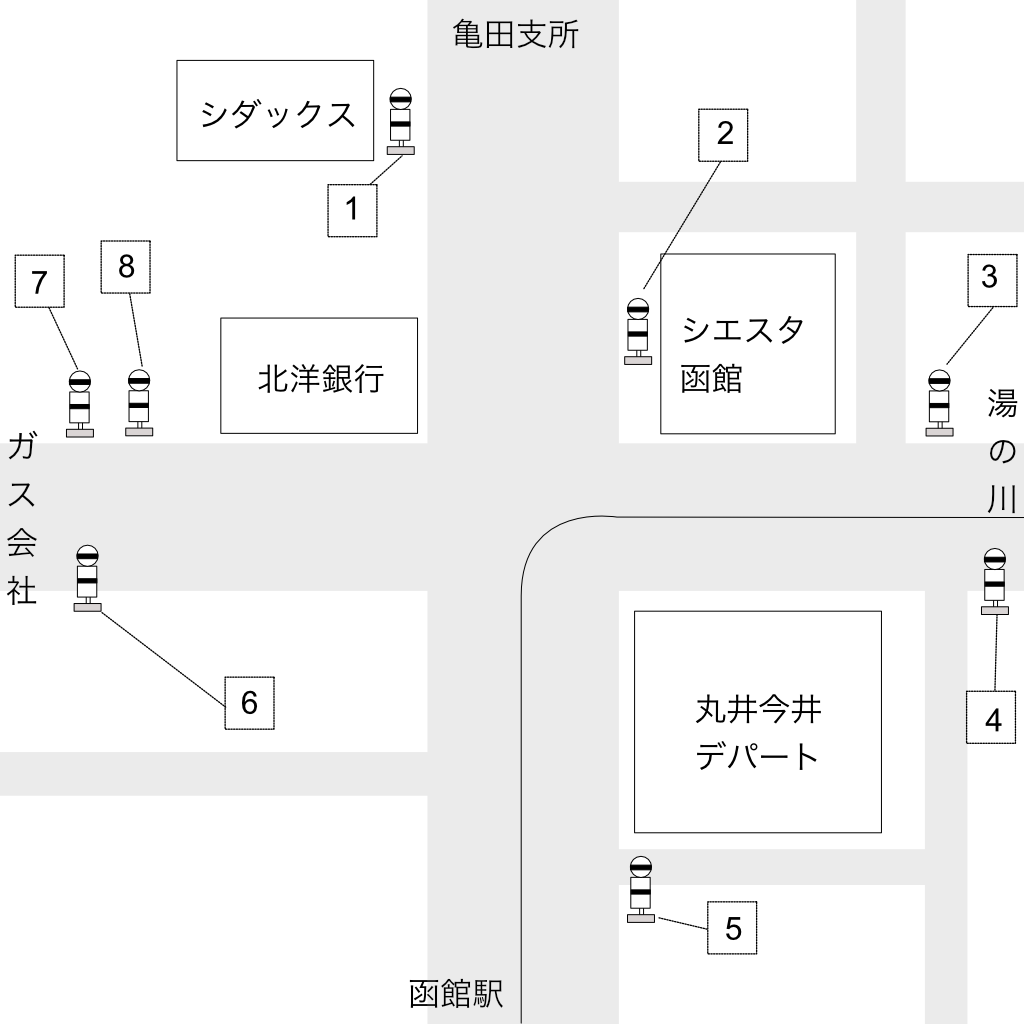
\includegraphics[clip,width=7.0cm]{img/14007.png}
    \caption{五稜郭バス停}
    \label{fig:goryo}
  \end{center}
\end{figure}

\chapter{Hako-Bについて}

\section{Hako-Bの概要}
Hako-Bは、ターゲットを函館のバスを初めて使う観光客へ向けたサービスである。
初めて函館に来た観光客でも迷うことなく函館のバスに乗ることができれば、地元の方にも分かりやすいサービスとなるため、観光客にターゲットを当てた。
函館のバスの分かりづらい点として、3.2項であげた問題のほか路線が完全に一致しているが往路と復路で別系統となっている路線も存在する。
そのため、系統番号だけでは判断できない。
それらを解決するために私たちはHako-Bを提案する。
Hako-Bとはバスとバス停にビーコンを設置し、ユーザーが乗車予定のバスの系統番号や行き先情報を既存のシステムや時刻表を見ずに乗車できることを目的としたアプリケーションサービスである。
\bunseki{北原康太}


\section{Hako-Bの機能}
観光客がHako-Bアプリケーションを起動すると、GPSを用いてマップから降車位置を選択でき、降車位置決定後、現在位置の周りにあるバス停を選択できる。
その後、現在位置から乗車予定のバス停までの経路表示をする。
乗車予定のバス停に近づくと、バス停に設置してあるビーコンから「乗車予定のバス停に近づきました」というPush通知が送られる。
さらに、近くにバス停が複数ある場所でも、迷わず乗車するバス停へたどり着くことができる。
そして、バス停に乗車予定のバスが到着した際には「乗車するバスが到着しました。バスに乗ってください」というPush通知が送られる。
そのため、複雑な系統番号や降車地が書かれていないバスでも間違うことなく正しいバスに乗ることができる。

\bunseki{北原康太}

\subsection{機能一覧}
本アプリケーションの機能は、主に5種類の機能がある。以下にそれぞれの機能について述べる。
\begin{enumerate}

\item バス停の選択\mbox{}

函館のバスが抱える1つ目の問題点として、観光や仕事などで初めて函館に来た人は以下の課題に直面する。
それは名前や位置など、紛らわしく分かりにくいバス停が多いということである。
例えば、赤川というバス停がある。
赤川という場所にあるバス停は赤川入口、赤川小学校前、赤川貯水池などのように赤川という名前が入っているバス停が3つ存在している。
函館になれていない人にとっては紛らわしい。
そこで、乗車するバス停を選択する際にマップからバス停を選択できるようにした。(図\ref{fig:select})
これによって函館へ初めて来た人にも使いやすくなるようにした。
また、マップからバス停を選択できるのでバス停の名前が複雑な場合も乗車地を選択しやすい。
しかし、バス停を設定する際にいくつもバス停がある場所であると設定することが難しい。
そのため複数のバス停がある五稜郭、函館駅前についてはマップ上にピンを1つしか建てない。
観光案内などでバス停の名前は分かるが位置を知らない場合には検索をすることでバス停を絞り込み、場所が分かるようにした。

\item 経路表示\mbox{}

名前や位置など、紛らわしく分かりにくいバス停が多い、という問題の解決のために経路を表示した。
位置が分かりにくい、という問題点の例として、五稜郭があげられる。
五稜郭のバス停は五稜郭の周辺に8つ存在しており、どの施設の前にあるか、という違いによって名前が違う。
このようにバス停が多く、しかも交差点を跨いで存在していると位置が分かりにくく初めての人は目的のバスを逃してしまう可能性がある。
そこで本アプリケーションには経路表示の機能を入れた。経路表示機能によってバス停までの道のりが分かるようになった。
経路は現在地からユーザーが設定した乗車地までを赤くマップ上に表示する。(図\ref{fig:root})
また、最短距離を表示するものとした。
経路表示をもとにバス停の近くへ行くとアプリケーションから通知が来てバス停が正しいかが分かる。

\item バス停の正誤判定\mbox{}

函館のバスが抱える2つ目の問題点として、函館では同じまたは似ている名前のバス停が複数存在している、という課題がある。
例えば、函館駅前のバス停は1番乗り場から7番乗り場まであり、その次は13番乗り場となっている。
これは普段使わない人にとってはどのバス停を使えば良いのか分かりにくい。
さらにこれらのバス停はお互い近くに存在しているので経路表示では十分な表示をできない可能性がある。
そこで私たちは、バス停に設置されているビーコンの電波範囲内に入った際、アプリケーションがユーザーに通知を行うようにした。
近づいたバス停が乗車地に設定したものであった場合は正しいという通知を行う。
同じ、または似ている名前のバス停が近くに存在する場合、乗車地に設定していないバス停に近づくと誤っているという通知を行う。
この通知によって、同じ、または似ている名前のバス停が複数存在していてもユーザーは迷うことなく設定したバス停を見つけることができる。
また、このバス停判別機能はビーコンの局所性を最も活用している機能である。
GPSによる測位では誤差が大きく、300m近くの誤差が生まれることもある。
この誤差の範囲内にバス停が複数存在した場合バス停を正確にユーザーに通知できない。
しかしビーコンは誤差が大きい場合でも数メートル程度のためバス停を正確に検知できる。

\item バスの通知\mbox{}

函館のバスが抱える3つ目の問題点として、目的地に行くためのバスの系統が分かりにくい、という課題がある。
例えば、はこだて未来大学へ行くバスには105,55,55-1という3つの系統がある。
このように同じ目的地でも複数の系統が存在している。
この問題を解決するため、設定した降車地へ行くバスが接近した際にユーザーへ通知を行うようにした。
目的のバスが接近し、ビーコンの電波範囲内に入った際、通知を行う。
設定していないバスが接近したときには通知を送らないようにしている。
函館のバスは系統が多いが、本アプリケーションからの通知によって、バスの系統表示を気にすることなくユーザーはバスを利用できる。

\end{enumerate}

\bunseki{小島雄士}


  \begin{figure}[H]
    \begin{tabular}{cc}
      %---- 最初の図 ---------------------------
      \begin{minipage}[t]{0.45\hsize}
        \centering
        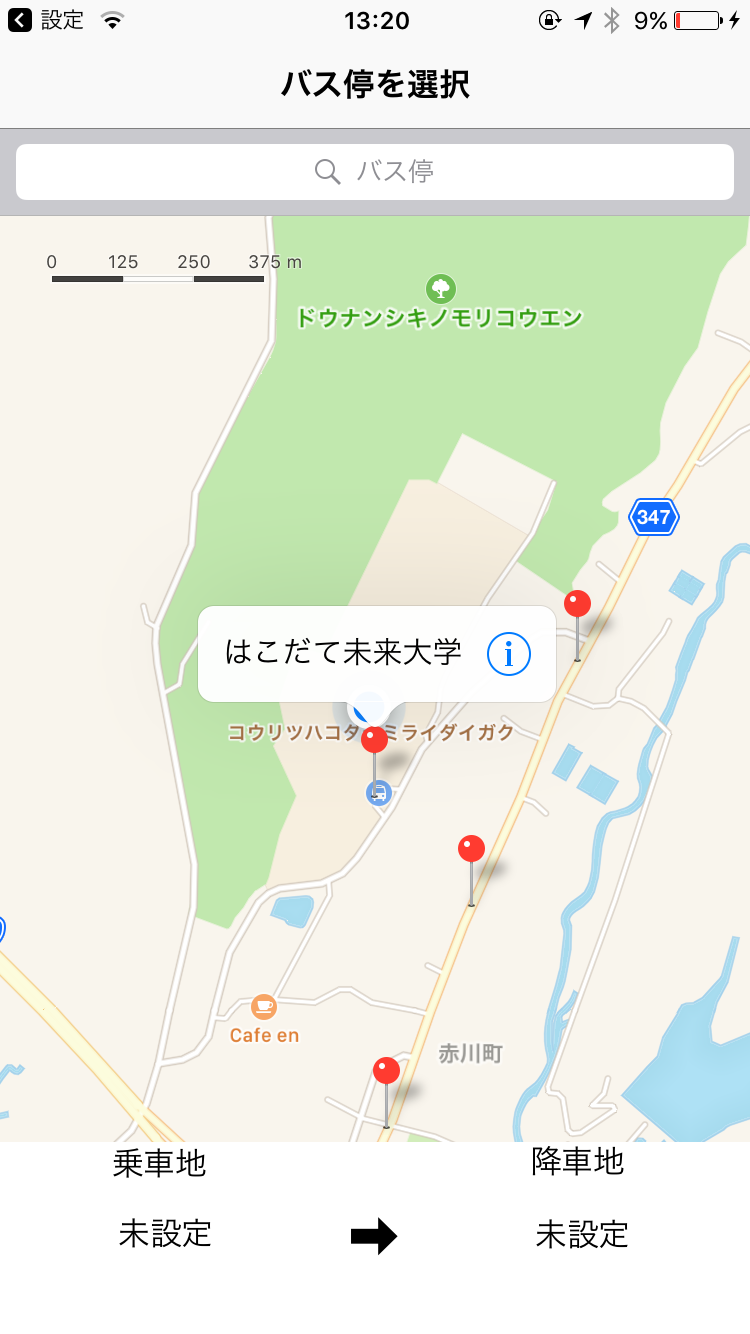
\includegraphics[keepaspectratio, scale=0.2]{img/select.png}
        \caption{バス停の選択}
        \label{fig:select}
      \end{minipage} &
      %---- 2番目の図 --------------------------
      \begin{minipage}[t]{0.45\hsize}
        \centering
        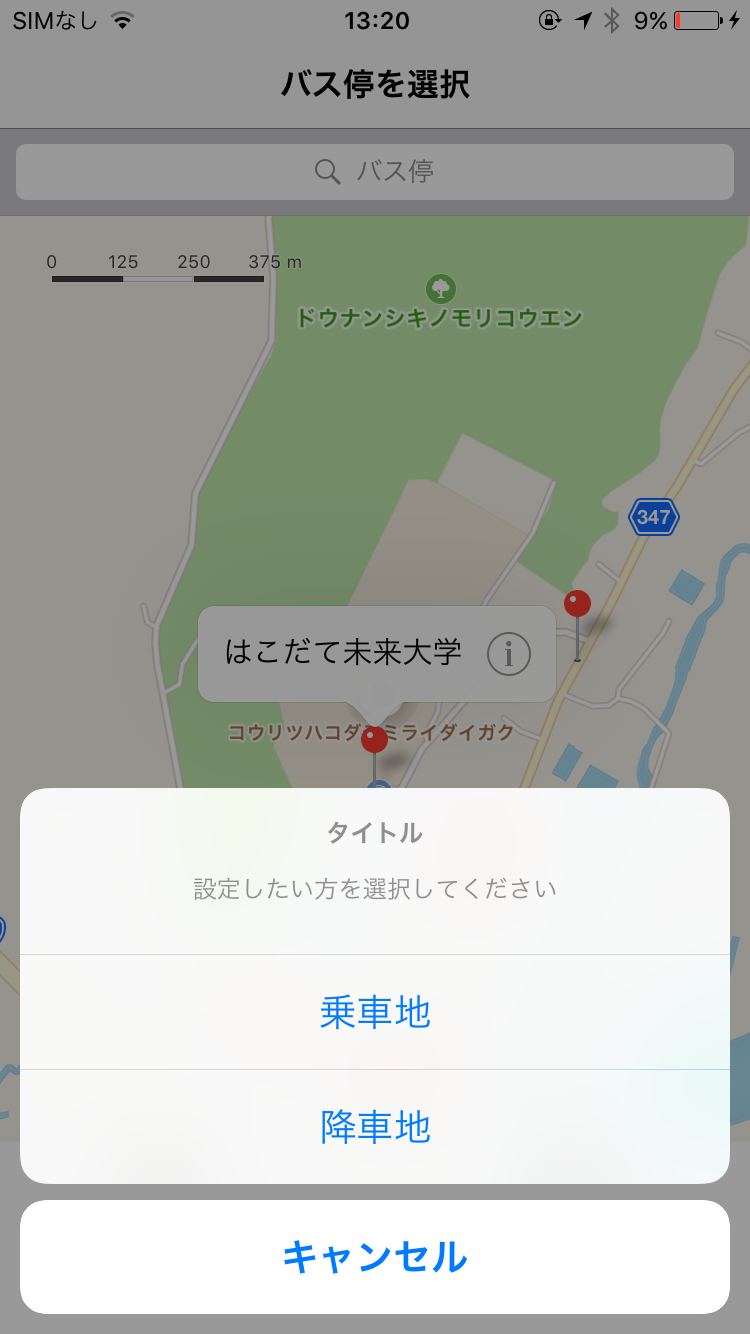
\includegraphics[keepaspectratio, scale=0.2]{img/select_bus.png}
        \caption{選択時のメニュー}
        \label{fig:select_bus}
      \end{minipage}\\
      %---- 3番目の図 --------------------------
      \begin{minipage}[t]{0.45\hsize}
        \centering
        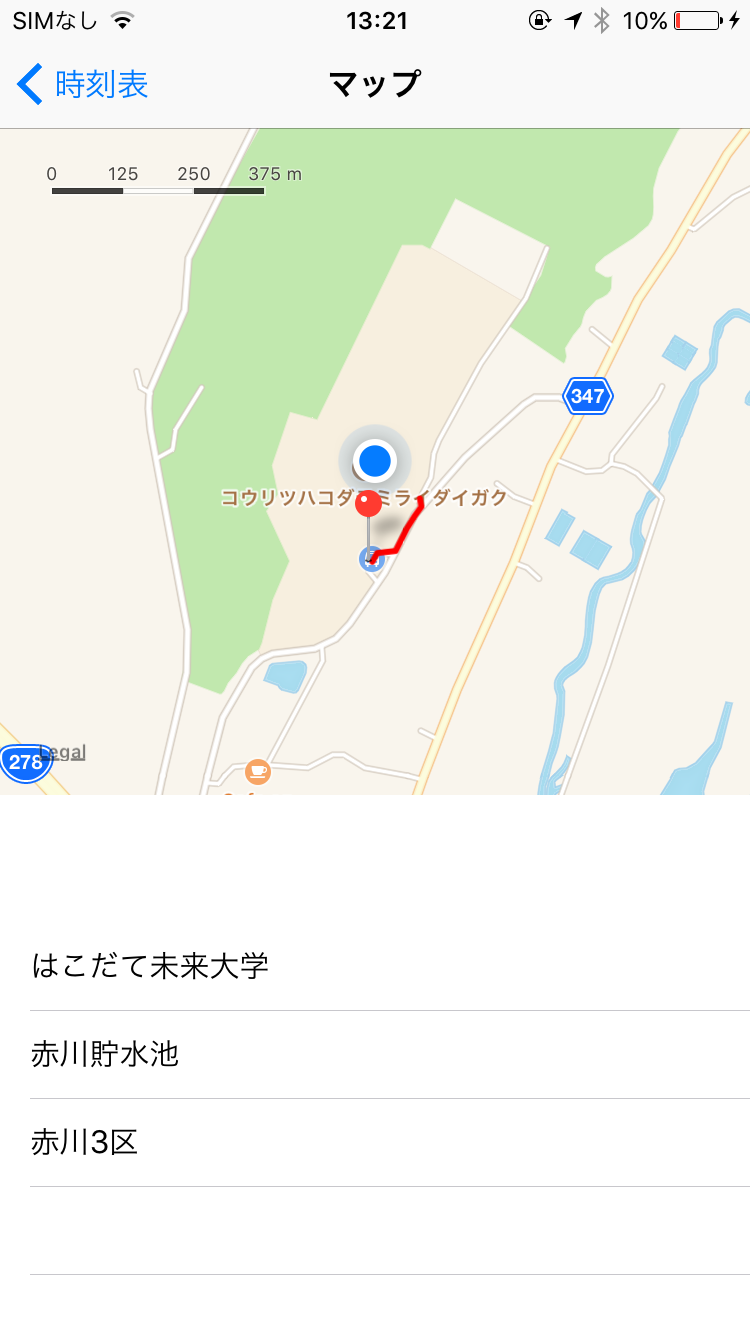
\includegraphics[keepaspectratio, scale=0.2]{img/root.png}
        \caption{経路表示}
        \label{fig:root}
      \end{minipage}\\
      %---- 図はここまで ----------------------
    \end{tabular}
  \end{figure}

\chapter{課題解決のプロセス}
\section{本グループの目標}
本プロジェクトにおける目標は、ビーコンを用いて函館のバス利用をより快適にできるようなアプリケーションを作成することである。
私たちでは「Hako-B」のアプリケーションでバスとバス停の判別をでき、乗り間違いを少なくできるような提案、開発をすることを目標とする。

\bunseki{佐藤秀輔}

\subsection{前期活動における目標}
前期の活動での目標は、開発するアプリケーションを使用し、どのように函館のバスの利用を快適にできるのかを考える。
そして、後期の開発へ向けアプリケーション機能の洗い出し設計を行うことである。
そのため、函館のバスを利用する際にどのような点が不便であるか、またビーコンを用いてどのような問題点を解決できるかを考え、アプリケーションに実装する機能を決める。
後期での開発を円滑に行うため、実装する機能を基にどのような画面遷移をするか、どのようなシステムにするのかを考え、画面遷移図などを作成する。

\bunseki{佐藤秀輔}

\subsection{後期活動における目標}
後期活動での目標は、前期活動にて考案した機能を実装したプロトタイプを作成し、実証実験まで行うことである。
作成したプロトタイプは、実証実験の前にビーコンを用いた基礎的なテストを行う。
また、メンバー内で実際にアプリケーションの使用の流れを確認しながらより使いやすいものになるようにレビューを行っていく。

\bunseki{北原康太}

\subsubsection{アプリケーションの作成}
前期活動にて考案した機能を基にアプリケーションの開発を行っていく。
アプリケーションに実装する機能は以下のものである。
\begin{itemize}

\item バスの時刻表情報
\item マップ上でのバス停の選択
\item バス停までの経路案内
\item バス停の正誤判定通知
\item 乗車予定バスの通知

\end{itemize}

作成したアプリケーションを実際に使用しどのような機能が使いづらいのかを確認する。
その後、その機能についてメンバー内で話し合いを行い機能の修正を行う。
このような流れを繰り返し、アプリケーションの作成を行っていく。

\bunseki{北原康太}

\subsubsection{基礎テスト}
前期の活動では実際にビーコンを用いたテストを行えなかったためビーコンを用いたテストを行った。
テストを行う際にある程度の精度があるかを確認するため以下の方法でテストを行った。

\begin{itemize}

\item 利用者がどの程度の距離まで接近すると通知が来るのか
\item ガラス越しで通知機能が起動するのかどうか

\end{itemize}

これらのテストではビーコンを起動しておき、どの程度の距離まで離れた際に通知が送られるのかを検証する。

\bunseki{佐藤秀輔}


\subsubsection{実証実験}

具体的な実証実験の方法としては、バス車内に設置されたビーコンと見立てて実際のバスへビーコンを持って乗車する。
バス停に立っているHako-Bアプリケーション利用者にバス接近情報が通知されるかどうかを確認する。
また、バス停付近にビーコンを持って立ち、どの範囲なら乗車予定のバス停がビーコンによって見つけられるかという点を検証する。
その際のテストでは、
\begin{itemize}

\item 実際にどの程度の距離よりビーコンの電波を検知してPush通知が送られてくるのか
\item 車内からのビーコンの電波でどの程度の距離から判別できるのか
\item バスが連なってきた場合のバスの判別
\item バス停が多くある箇所で目的のバス停が判別できるのか

\end{itemize}
これらのビーコンが用いられている箇所の動作を安定させるようなテストを行う。

\bunseki{北原康太}


\section{サービス設計}

\subsection{システム概要}
本システムは、バスとバス停に設置されたビーコンにより、そのバスとバス停の正誤判定をするというシステムである。
主な機能としては、目的のバスとバス停へ近づいた際にPush通知を送るというものである。
また、Push通知を送るだけでなく近くのバス停をマップから選択する。
その後、時刻表などを確認でき、利用者が簡単にバスの情報を集めることができる。

\bunseki{佐藤秀輔}

\subsection{ユースケース}
システムとユーザー間でどのような処理が必要になるのか確認するためにユースケースを作成した。
作成したユースケースを基にユースケース図を作成した(図\ref{fig:usecase})。
アクターである観光者はアプリケーションを起動し、目的地、現在地付近のバス停を選択する。
選択したのち、ユーザーが選択したバス停のビーコンの範囲内に入るとPush通知を受け取る。
その後、目的地まで向かうバスに設置されたビーコンの範囲内に入るとPush通知を受け取る。

\begin{figure}[htbp]
  \begin{center}
    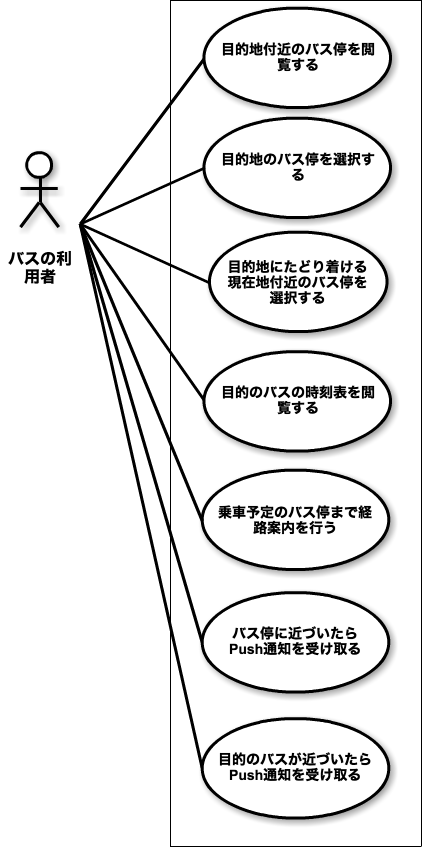
\includegraphics[clip,width=5.0cm]{img/usecase.png}
    \caption{ユースケース図}
    \label{fig:usecase}
  \end{center}
\end{figure}
\bunseki{佐藤秀輔}


\section{環境構築}
各メンバーとの連絡はSlackを用いて行った。
Slackでは、グループメンバーへの連絡、一部ファイルなどの共有に利用した。
私たちはiOSのアプリケーションを開発するためAppleが提供しているXcodeという統合開発環境を使用した。
Xcodeを使用するためにまずはApple IDの作成が必要だったため個人の持っているアカウントもしくは開発のためにAppleアカウントを作成を行った。
開発の環境としてはXcodeのインストールを行うことで整うためXcodeのインストールを行った。
また、Xcodeを用いてアプリケーションを作成する前にProttというプロトタイピングツールを用いてプロトタイプの作成を行った。
GitHubでは、リモートリポジトリに機能の追加、バグの修正などの種類ごとでブランチを作成し、リモートブランチへプッシュした。
developなどの開発用のブランチを作成せずmasterにマージするとき、テストを行い問題がないかレビューを行いmasterへマージをするという手法で行った。
masterにマージする際、レビューを徹底することでmasterのファイルでバグが起きないようにできる。

\bunseki{佐藤秀輔}

\subsection{Xcode}
今回のアプリケーション開発ではAndroid、iOSの両方の開発をすることが難しいためiOSのアプリケーション開発を行うこととした。
そのためアプリケーション開発には、Apple社が開発したXcodeという統合開発環境を使用して開発することにした\cite{Apple}。
開発言語はSwiftを使用した。
使用したバージョンはXcode8.3、Swift3.0の環境で開発をした。
XcodeにはInterfaceBuilderという機能があり実際にコードを書かなくても視覚的にUIを作成する機能があり、リファレンスなど充実しているため開発ツールにXcodeを選択した。
また、Xcode上でシミュレータを起動し実際にiPhoneで動かしているかのようなデバック機能があるため実際にiPhoneを持っていたりしなくても現在のコードを確認できるというメリットも有る。

\bunseki{佐藤秀輔}

\subsection{Prott}
プロトタイプの作成のために株式会社グッドパッチが提供するProttというプロトタイピングツールを用いた\cite{Prott}。
アプリケーションの開発前にプロトタイプを作成することでメンバー間でのアプリケーションに対する情報共有を行った。
このプロトタイプでは、実際の位置情報やバス停の位置情報などは取得できていないが全メンバーでアプリケーションの動きなどを確認できた(図\ref{fig:prott})。
前期時点で考案していた機能に関しては作成してあったため実際の開発ではこのプロトタイプを参考に開発を進めていった。

\begin{figure}[htbp]
  \begin{center}
    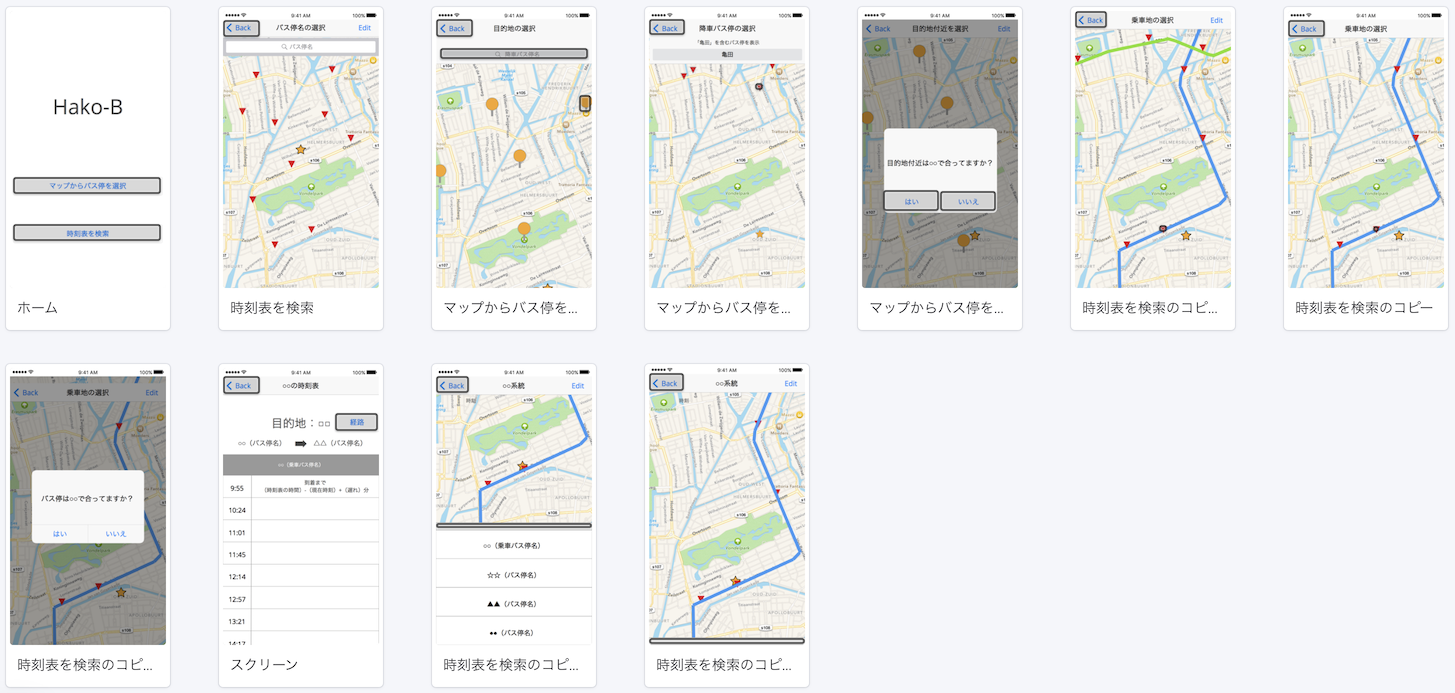
\includegraphics[clip,width=\hsize]{img/prott.png}
    \caption{プロトタイプ}
    \label{fig:prott}
  \end{center}
\end{figure}

\bunseki{佐藤秀輔}

\subsection{Git/GitHub}
ソースコードのバージョン管理ツールとしてGit/GitHubを使用した。
Gitは分散型のバージョン管理システムの1つであり、すべてのファイルの変更履歴を含む完全なリポジトリの複製を保存できるというものである。
その為、一度編集したファイルを基に戻すことやどのような編集が行われたのか表示することが可能となる。
リポジトリにはネットワーク上に保存されているリモートリポジトリと、メンバーそれぞれのPC内に保存されているローカルリポジトリの2種類がある\cite{b}。
リモートリポジトリではメンバーそれぞれのファイルの変更履歴を保存し確認、共有できる。
GitHubとはリモートリポジトリを提供するサービスの1つである。
GitHubを使用することにより、複数のメンバー間でスムーズにファイルを共有し開発することが可能となった。

\bunseki{佐藤秀輔}

\section{技術習得}
メンバー全員でiOSのアプリケーション開発経験のある人が1人しかいなかったため、夏季休業期間中にアプリケーション開発の基礎的な知識を学習できるような資料の作成を行った。
メンバーには作成した資料に基づき、経験のあるメンバーに質問をしながら基礎的な知識をつけられるように活動を行った。
夏季休業期間期間ではメンバー同士で集まることが難しかったため各自、作成された資料を見ながら個人で進めていった。
その際のプログラムの教材として
\begin{itemize}

\item Swiftの基礎知識
\item Hello Worldのプログラム作成
\item TableViewを用いたアプリケーションの作成

\end{itemize}
の3つを題材として基礎的な知識について学習を行った。
プログラムの教材に関しての質問は今回資料を作成したメンバーをメンターとし、出てきた質問に対応してもらった。

\bunseki{佐藤秀輔}

\section{中間発表会}
\subsection{発表形式}
始めにメインポスターの発表を5分間行った後、聞き手には3つのサブポスターのどれかを選んでもらいそれぞれ発表を聞いてもらった。
Hako-Bのポスターセッションでは前半と後半それぞれ2人ずつに分かれて発表を行った。
1人は概要、システム構成、今後の予定を話し、もう1人はHako-Bについてを話した。

\bunseki{小笠原瑠奈}

\subsection{発表内容}
始めに、概要を説明した。
まず、Hako-B を提案するに至った問題点を実際のバス停の例と画像を用いて提示した。
1 つ目は同じバス停名が近くに複数存在すること、2 つ目は似たような名前のバス停が存在すること、3 つ目は目的地に行くためのバスの系統がわかりづらいことだった。
その後、先に述べた問題から生じるミスを解消することを目的として示した。
次に、Hako-B の機能説明をした。
まず、アプリケーションの特徴を箇条書きで大まかに示した。
特徴は3 つあり、1 つ目は利用者が設定したバス停までの道案内をGPS を用いて行うことである。
2 つ目はバス停に設置されたビーコンから受けた電波によってバス停への接近を利用者に通知することである。
そして3 つ目は、バスの車内に設置されたビーコンから受けた電波によってバスの到着を通知することである。
その後、処理フローでイラストやスマートフォン画面などの画像を用いてアプリケーションの機能を具体的に説明した。
次に、システム構成の説明を行い、今後の予定を3 つ示した。
1 つ目は設計を基にプロトタイプを作成することである。
2 つ目は模擬バス、模擬バス停による実証実験を行うことである。
3 つ目はテストで出た問題の改善を行うことである。
以上がポスター発表の内容となる。

\bunseki{小笠原瑠奈}

\subsection{レビュー内容}

\subsubsection{発表方法についての評価と反省}
発表方法に関して、プラスの意見として
\begin{itemize}

\item 身振り手振りがあって良い
\item 発表が分かりやすかった

\end{itemize}
などが挙げられ、聞き手に内容を上手く伝えることができたと分かる。以上から発表技術に問題はなかったと言える。
マイナスの意見としては
\begin{itemize}

\item 声が聞き取りづらい
\item ポスターのレイアウトが意味不明
\item 画面遷移図が小さい
\item 図に少し説明を入れると良い

\end{itemize}
などが挙げられた。平均評価は7であった。
以上から、
\begin{itemize}

\item 発表する際の各グループの配置や向きを見直す必要がある
\item ポスターのレイアウトを読み進めやすいものにする
\item アプリケーション画面のテキストをポスター用に大きくする
\item 図を見やすくして説明を付ける

\end{itemize}
上記の4つが改善点として挙げられる。

\bunseki{小笠原瑠奈}

\subsubsection{発表内容についての評価と反省}
発表内容に関しては、プラスの意見として
\begin{itemize}

\item 問題の着目点が良い
\item アプリケーションのニーズは高い
\item 実際に欲しい

\end{itemize}
などが挙げられた。
以上より、提案に対する聞き手のニーズが高いと分かった。
マイナスの意見としては、
\begin{itemize}

\item プロトタイプもできていないので課題が山積み
\item 内容の検討がたりない
\item ビーコンの利点をうまく使いこなせていない。もっと他にも良い活用法があるかもしれない
\item バス停名が分からない人にはどうするのか
\item 計画を具体的に詰めたら良い

\end{itemize}
などが挙げられ、提案システムの問題点や今後の予定が詳細に決められていないことに指摘を受けた。
平均評価は7であった。
以上から、今後出来るだけ早い段階からプロトタイプを作る必要があること、様々なアクターを想定したユースケースを再検討すること、今後の計画を詳細に決めることが改善点として挙げられる。
また、「バス停名が分からない人にはどうするのか」という指摘に対しては、ユーザーが目的地を入力するとマップ上から推奨される降車地と乗車地を選択できるというアプリケーションの機能が解決策となる。
しかし、これは展望であり、実装予定の機能としてはポスターに載せていなかったので説明不足であったと反省する。

\bunseki{小笠原瑠奈}

\section{オープンキャンパス}
はこだて未来大学のオープンキャンパスで本プロジェクトの説明を行った。
説明方法はオープンキャンパスに来た方々がポスターの前に立ち止まり見ているときにHako-Bについての説明を行う、という方法をとった。
また、ポスターは大学生や先生を対象としたポスターになっているためオープンキャンパスへ来た方々には難しい用語がある。
そのためポスター説明で専門用語を話す際にはその都度用語の説明をした。

\bunseki{小島雄士}

\section{デモ発表会}
プロジェクト内での各グループの進捗を確認を行うためにでも発表会を行った。
デモ発表会では、成果報告会と同じ形式で行うため開発と同時にポスターの作成も行った。
この時プロジェクトの教員3名より作成したアプリケーションとポスターに関してコメントを頂いた。

\bunseki{佐藤秀輔}

\subsection{内容}
開発したアプリケーションのUI、機能などの意見をもらうため私達のプロジェクトの教員方に発表を行った。
発表会ではポスター、実機を用いて説明を行った。
最初にポスターの説明を行った。
デモ発表会のため、ポスターの説明は簡略化して行い、デモの説明を多くした。
まずHako-Bの概要を説明した。
その後、実機の画面をプロジェクターで投影してデモを見せながらアプリケーションの機能を説明した。
前期のポスターとの違いとして、既存のアプリケーションとの差別化をした点を新しく入れた。
デモ発表会の時点ではまだ、経路表示、乗車地に設定していないバス停についたときの誤り判定はなかった。

\bunseki{小島雄士}

\subsection{レビュー}
デモ発表会のレビューは「デモの完成度は高かったですか」「ポスターはわかりやすかったですか」の2項目に分けてレビューを行った。
それぞれ、「わかりにくかった」から「わかりやすかった」まで5段階で評価を受けた。
また、それぞれ改善点やコメントをした。

デモに対しての評価としては5段階評価で平均3.3となった。
コメントには以下のようなものがあった。
\begin{itemize}

\item この時期にしてはかなり進んでいる状態だと思います。ただ、もっと欲を言うとUIにこだわれるようになるといいと思います
\item 機能も見た目も割と出来ているように見えました
\item 亀田支所や五稜郭前など分かりやすい場所のデモをするとわかりやすい
\item 複数個バス停があるので乗りやすいというのがアピールポイントだと思うので、早めに経路表示を実装した方がいいと思います
\item もう少しストーリー性があると良いと思った

\end{itemize}

以上のコメントより、アプリケーションの機能面に関しては実装が進んでいる。
また、アプリケーションの見た目に関しても分かりやすいものになっていると思われる。
デモの改善点としてはより分かりやすいデモを行うことが必要である。
コメントにあるように、亀田支所や五稜郭を使用してデモを行うと分かりやすく感じた。
そして、経路表示の実装を早めにすると説明も分かりやすくなる。
また、初めてHako-Bを初めて見た人に対して、アプリケーションの有用性を説明することも大切だと思われる。
今回は同じプロジェクト内でのレビューなのである程度概要を知っている状態でレビューをした。
しかし、初めて見る人に対してはビーコンをどこに使っているのか、どのような流れでアプリケーションを使えばいいのかといったHako-Bの説明がまだまだ足りていないと思われる。

ポスターに対しての評価としては5段階評価で平均3.3となった。また、コメントには以下のようなものがあった。
\begin{itemize}

\item 全体的に見やすかった
\item 機能ごとに画面を表示しているのが良い。既存のアプリケーションとの違いの欄に不自然な空白があるのが気になった
\item 人が物事を理解するときは、Whyの説明がかなり重要です。機能が必要な理由を述べられると良いです
\item 目的や背景がないので動機が分かりづらい
\item 全体的に図と説明が足りない。ポスターからはHako-Bの魅力が伝わらないので、Hako-Bとはの部分をもう少し説明を濃くした方がいいかもしれないです。もしくは、全体の流れを表す図を入れた方がいいと思います
\item テキストが多いと感じた

\end{itemize}
以上のコメントより、作成したポスターはシンプルだったと考えられる。
デモの改善点としては主に見た目に関してのものが多かった。
例えば図が少ない、不自然な空白がある、テキストが多いなどがあげられる。
また、目的や背景を入れていなかったため、動機が分かりづらい、というコメントもあった。
「Hako-Bの機能が必要な理由が足りていない」「Hako-Bについての説明が少ない」などのコメントより、デモと同じようにアプリケーションについての説明が不十分だったと考えられる。
アプリケーションの図もただ4つあるだけだと順番に並んでいても気が付かないので矢印や数字などを使って見やすくするように改善したい。

\bunseki{小島雄士}

\section{プロジェクト学習見学者への発表}
2017年12月6日に来ていただいた金沢工業大学の教授の方々に向けてポスターを使用して発表した。
時間が限られていたため3分程度で説明をした。
まず、Hako-Bの概要を説明した。
その後簡略化してアプリケーションの使用フローやアプリケーション画面を説明した。
最後に今後の展望を発表した。
発表では時間が限られていたためゆっくりと時間を取って詳しく話すことができなかったがビーコンを使うことの有意性、要点など十分に発表できた。

\bunseki{小島雄士}

\section{成果報告会}
\subsection{発表形式}
始めにプロジェクト全体の発表をスライドで5分間行った後、聞き手に3つのサブポスターのどれかを選んでもらい発表を聞いてもらった。
Hako-Bのポスターセッションは中間発表会と同じ形式で、発表者の組み合わせも同じであったが、同時にアプリケーションのデモを行った。
1人は問題、Hako-Bについて、アプリケーションの使用フローや学び、展望を話した。
もう1人はアプリケーションの機能について実際にアプリケーションを動かして説明した。
デモではアプリケーションがバスとバス停のビーコンを検知することに重点を置いてデモを行った。
その中では、アプリケーションを動かすほうがバス停のビーコンを持ち、もう1人がバスのビーコンを動かすことでPush通知が来る様子を見せた。

\bunseki{小笠原瑠奈}

\subsection{発表内容}
まず概要において、アプリケーションを開発するに至った背景として以下の3点を函館バスの問題点であると例えを交えながら提示した。
初めて函館に来た人はバス停名・位置が分かりづらい。
函館では同じまたは似たような名前のバス停が複数ある。
目的地に行くためのバスの系統が分かりづらい。
以上の3点を函館のバスの問題点であると、例えを交えながら提示した。
その後、提示した問題を解決するために開発したという流れでHako-Bとはどのようなアプリケーションなのかを簡潔に説明した。
次にアプリケーションの使用フローを説明した後、分かりやすいよう実際にアプリケーションのデモを行った。
デモでは、マップから乗車地・降車地を選択した後、次の画面で時刻表をタップすると乗車地までの経路が表示されるという流れを軽く示した。
乗車地・降車地選択の画面では検索フォームに「赤川」と入力すると「赤川」が含まれるバス停だけが表示される様子も見せた。
そして、「はこだて未来大学」を想定したビーコンをスマートフォンに近づけると「バス停が近くにあります」、違うビーコンを近づけると「違うよ!」と通知される。
その後、バスを想定したビーコンが近づくと「バスが到着しました」と通知される様子を見せた。
最後に、後期の活動を経ての学びとして以下の2点を提示した。
SwiftでのiOSアプリケーション開発の流れを学んだ。
ビーコンを用いた局所的な位置情報の利用法を学んだ。
今後の展望としては以下の2点を提示した。
正確なバス遅延時間の表示を行う。
乗り換えも考えたルートの表示を行う。

\bunseki{小笠原瑠奈}

\subsection{レビュー内容}

\subsubsection{発表方法についての評価と反省}
発表方法に関して、プレゼンテーションに関するプラスの意見として
\begin{itemize}

\item 具体的なシチュエーションでの説明がわかりやすかった
\item とても効果的なプレゼンが出来ていました
\item 詳細をしっかり説明してくれている
\item 詳細をしっかり説明してくれている
\item 発表する速さが程度良い感じです

\end{itemize}

などがあった。また、ポスターに関しては
\begin{itemize}

\item ポスターの図が分かりやすかった
\item と内容をまとめられていたため分かりやすかった

\end{itemize}

などがあり、デモに関しては
\begin{itemize}

\item 発表技術について、体験ができて、理解しやすかった
\item デモを行っていてわかりやすい。大きめのディスプレイを使っていてわかりやすかった

\end{itemize}

などの意見をいただいた。次にマイナスの意見に関しては、
\begin{itemize}

\item 少し声が聞き取りにくかった
\item 声が小さく聞き取りづらかった
\item パネルセッションなのでパネルかくさない方がよいのでは?

\end{itemize}
など声の通りに対する意見を多くいただいた。
以上から、内容を説明する流れやポスター、デモは高評価であったことから分かりやすく、効果的であったと思われるが声量や動きに問題があったと言える。
平均評価は7.5で、中間発表会よりも0.5ポイント上がった。

\bunseki{小笠原瑠奈}

\subsubsection{発表内容についての評価と反省}
発表内容について、開発したアプリケーションに関するプラスの意見として
\begin{itemize}

\item はこだてのバスの問題をビーコンで解決しようとした点は、ユニークで面白いと思いました
\item アプリケーションのデザイン、とても良かった。これまでにない地域に合う案内方法ができると思いました
\item 市民の抱える問題に対する課題解決がテーマになっていて、わかりやすかった
\item Hako-B使ってみたいです。バスは乗らないのですが、このアプリケーションがあれば乗ってみようと思います
\item Beaconとてもおもしろそうでした。実用化されたら欲しい
\item アイデアは非常に面白く、欲しいと感じました
\item このアプリケーションが実装されたらもっと快適に乗ることができると思った

\end{itemize}
などの意見を頂いた。アプリケーション以外の事柄に関しては
\begin{itemize}

\item 次の課題も把握しているところが良いと思った
\item 利用の流れがわかりやすかった
\item メンバーの学びがあるのがよい

\end{itemize}
などの意見をいただいた。次にアプリケーションに関するマイナスの意見としては、
\begin{itemize}

\item その場所(土地)を全く知らない人にも、やさしいUIとサービスがあるとよいと思いました。(StartとEndがわかっている段階での話に感じました)
\item 実証実験などをもう少しやると、よいと思いました
\item 実際に実験をしてシステムとしてなりたつのかを是非確認してほしい!
\item アプリケーションで自分の行きたい目的地を指定してもよりのバス停を指定できるようにしたら良いと思います。(乗車地、降車地を指定してくれる)
\item 質問にあったように時間のずれが分かるといい

\end{itemize}
などの意見を頂いき、アプリケーション以外の事柄に関しては
\begin{itemize}

\item ビーコンとアプリケーションの関係性(どうやってリンク?させるか等)の説明がなかったので、もう少し動作の中身が知りたい
\item 学びの部分が苦労したことやどう解決したかなどが知りたかった

\end{itemize}
などの意見をいただいた。
以上からアプリケーションの有用性は高く、使いたいという意見も多かったことからHako-Bに対する評価は高いことが伺えた。
バス停の選択や時刻表などユーザー任せ、実現できなかった機能に対する指摘も多かったので今後の課題としたい。
アプリケーション以外では学び、展望に触れていることが好感触であった。
しかし、「もう少し詳しく説明してほしい」「アプリケーションのビーコンの連携など技術的なことに関する説明についても深く触れてほしい」という意見もあったので、詳細に説明すべきであったと感じた。
平均評価は8.5で中間発表よりも1.5ポイント上がっていた。

\bunseki{小笠原瑠奈}


\chapter{各メンバーの役割と活動の振り返り}
\section{役割分担}
私たちは、メンバー全員が開発をできるようにアプリケーション内の機能ごとで役割分担を行った。
開発にはXcodeを用いてHako-Bのアプリケーションの作成を行った。
まず、メンバー全員でどのような機能が必要かを話し合いその話あった結果を基に画面構成図を作成した。
その後、作成した構成図を用いて開発に取り組んだ。
メンバーの1人はメンターという立場となり、各メンバーが実装など、困った際は助けられるようにした。
11月からは、数名に成果発表会で使用するポスターの作成を行った。
私たちはメンバー全員が一度はアプリケーションに触り、機能が実装できることを目的とし役割分担を行った。
各メンバーの担当箇所は以下に示す。

\subsubsection{北原康太}
\begin{itemize}
  \item 画面遷移図の作成\\
    画面遷移に関してどのようにしたら良いのか意見を出し作成のサポートを行いながら作成を行った。
	\item Xcodeを用いた開発\\
    マップを使用した箇所の実装を行いマップ上でバス停の位置を確認できるようにした。
\end{itemize}

\subsubsection{佐藤秀輔}
\begin{itemize}
	\item 進捗管理\\
    メンバーがやるべきことを確認し、作業を行えるように助言も添えタスク管理を行った。
  \item 画面遷移図の作成\\
    メンバーと相談をしながらどのようなアプリケーションの流れであれば使い易いのか相談しながら作成を行った。
	\item Xcodeを用いた開発\\
    ビーコンを使用したアプリケーションの開発を学ぶことができた。
  \item 他メンバーのメンター\\
    他のメンバーがアプリケーション作成に関して初めてであったため、作業が止まったりしていた場合作業を手伝えるようにしていた。
  \item ポスターの作成\\
    他のメンバーがポスターを中心的に作成し、ポスターに対するレビューを行うなどをした。
\end{itemize}

\subsubsection{小笠原瑠奈}
\begin{itemize}
	\item Xcodeを用いた開発\\
    時刻表の表示機能の部分を中心的に行いバスが何分後に出てくるのかなどをTableViewで表示できるようにした。
  \item ポスターの作成\\
    ポスターの作成を中心的に行った。
  \item プロトタイプの作成\\
    Prottというプロトタイプ作成ツールを用いてプロトタイプの作成を行った。
\end{itemize}

\subsubsection{小島雄士}
\begin{itemize}
	\item Xcodeを用いた開発\\
    Map画面でのバス停のサーチ機能の実装を行った。
  \item ポスターの作成\\
    メンバーを補助しながら、ポスター作成を行った。
\end{itemize}

\bunseki{佐藤秀輔}

\section{北原康太}
問題点からその解決策を見出す難しさを身にしみて感じた。
特に、前期活動で行った「アイデアソン」や「アイデアコンテスト」の中で短い時間の中いくつものアイデアを紙に書き出した。
そして、創出した経験は今後の学生生活や実際の業務に携わったときにも役に立つ手段だと思う。
また、実際に大勢の人の前でプレゼンテーションをする機会が今までなかったため、中間発表や最終発表でのプレゼンテーションはいい経験になった。 
そして、チーム開発においては今まで扱ったことのないGithubを使用して、ソースコードの管理を行った。
Githubを使うときに苦労したのは、コンフリクトが起きてしまったとき、解消するために時間がかかった点だ。
その際に、お互いにコミュニケーションをとって相手の開発担当部分を理解するという学習が大いに自分のためになった。
人のソースコードを読んで理解しやすい点・しにくい点を参考にして自分のコードを見直すきっかけになれた。
これより、ユーザーの求める機能がなんであるかをメンバーと考えて開発に携われたことがチーム開発から得られた経験である。 
また、今まで扱ったことのない言語である「Swift」を使用して、バス停関係の開発を担当できた。
函館バスのWebサイトからバス停の緯度経度を取得し、アプリケーションのマップ上にバス停を立てた。
そして、何よりもビーコンというものを学べた点が一番大きい。
プロジェクト配属前にはビーコンはどいういうものかも知らなかったが、企業の方のレクチャーや各自でビーコンについて調べ物をし、みんなの前で発表するということを通じてビーコンについて知ることができた。
また、プロジェクトを通して反省するべき点も多く見つかった。
例えば、わからないことがあった場合グループリーダーへすぐに頼り過ぎてしまっていた点。
当初はバス停やバスの管理にサーバを立てて管理しようとしたが、そういった知識を持ったメンバーは1人もおらず、時間がかかりすぎるため断念してしまった点。
自分の実力不足から諦めてしまった点。
これらの3点が反省スべき点であった。
以上より、1年を通してビーコンの知識やiPhoneアプリケーションの開発方法、チーム開発の手法やその際に用いるツールなどを使って楽しく開発できた。 
これからも、プロジェクトで得た経験や知識を活かして、残りの学生生活や将来に向けて精進していきたい。 

\bunseki{北原康太}

\section{佐藤秀輔}
今回のプロジェクトでは函館という1つの地域に目を当ててどこに問題があり、その問題をどのようにビーコンを用いて解決をするのかということを考えるというところが初めての経験だった。
私は、このグループAのグループリーダーとして活動していたがメンバーをまとめ、メンバーごとに指示を出したりするということがかなり難しいと感じた。
活動の中でグループのメンバーへの指示が遅くなったり、あまり指示を詳しく出すことができていなくメンバーの作業が止まってしまうことがあり、その部分を改善しなければいけないと感じた。
開発に関しては、今回のiOSアプリケーションの開発で自分しか開発経験がなかった。
そのためメンバーがアプリケーション開発の基礎知識をつけられるように、Swiftの資料などを作成するということをした。
成果発表では、自分たちの作成したものがどのように有用なのか、どうしてこのアプリケーションが必要なのかという点を伝えられた。
その結果、成果報告会では「このアプリケーションを使いたい」とのコメントを頂けた。
反省点としては、UIに関してあまり力をかけることができなかったため「UIがわかりづらい」とのコメントがあったのでUI改善を行っていきたい。
今回のプロジェクト学習を通して、リーダーとしてどのようにメンバーに指示を出していくのか、iOSアプリケーションでのビーコンの扱いの仕方などを学ぶことができ良い経験を得ることができた。

\bunseki{佐藤秀輔}

\section{小笠原瑠奈}
サービスを提案して、反応が得られる面白さが印象に残った。
特に、中間発表会では提案するアプリケーションやポスター・発表方法について多くの指摘を受けた。
しかし、成果報告会では「アプリケーションを使いたい」「分かりやすい説明」などの肯定的な反応を多く得られたのが嬉しかった。
また、サービスの提案から設計、開発までの一連の流れを体験できたのは学びとなった。
具体的には、フィールドワークやアイデアソンなど課題発掘やアイデア提案の手法を学ぶことができた。
加えて、チーム内での話し合い、コミュニケーション、作業の分担、連携など複数人で取り組む難しさを実体験できた。
技術面に関してはあまり上達感を得られなかったがSwiftと、Illustratorに関して扱う技術を身につけた。
一方、グループ活動を通して実感した反省も多かった。
「課題発掘における関心や経験の無さ」「多角的に見ることが上手くなかったためにアイデアの問題点を多く発見できない」「コミュニケーションが足りないので連携が取れない」などがある。
以上から、プロジェクト学習を通してサービスを提案する楽しさと難しさ、チームで開発することによる多くの反省を得た。
今後はこれらの反省点を改善し、学んだことを卒業研究など今後の活動に活かしていきたい。

\bunseki{小笠原瑠奈}

\section{小島雄士}
個人の振り返りとしてはSwiftを使用したアプリケーション開発、Gitの使い方、ビーコンという新しい技術について学ぶことができたのは大きい。
まず、Swiftを使用したアプリケーション開発を行うことができたのは良い経験となった。
Swiftという今までに使用したことのない言語を学ぶ機会が得られた。
今まではアプリケーションの開発というものをやったことがなく、漠然としたイメージしかなかった。
また、今までに制作したものは全て機能が1つのものだけだったため、本プロジェクトによってアプリケーション開発を経験できたのはいい機会であった。
次に、Gitを使用できたことも今後の糧となる。
プロジェクト開始以前はGitを使用したことがなく、知識もなかった。
しかしプロジェクト内の講習会や開発によってGitについての理解を深めることができた。
Gitを使用した開発においては、コンフリクトや役割分担などで苦労した。
今までは1人でソースコードを書く機会しかなかったため、チーム開発でのみ起こりうるこれらの苦労を経験することは良い経験となった。
チームでの開発は行ったことがなくチーム開発の大変さや苦労を経験できた。
細かく連絡や進捗の報告をすることがとても大変であり大切なことだと気づくことができた。
将来チームで開発を行う機会はあると思うので、今回の経験を生かしたい。
また、ビーコンという技術に触れることができ、自分の知らなかった知識を得ることができた。
プロジェクト開始以前はビーコンについての知識がほぼなかったがビーコンについて調べ、プロジェクト内での話し合いなどを通して知識を得ることができた。
ビーコンがどのような情報を持った端末なのか、なにができるのかなどを知ることができた。
今後ビーコンなどの位置情報を利用した開発を行う際に今回得た知識を生かしたいと思う。

反省として、ビーコンの端末についての知識を得ることができたが開発に関しては知識が足りなかった。
Swiiftを使用してビーコンから情報を得る方法については完全に理解をできず、コードを書くことができなかった。
今後はビーコンを使用する際にビーコンの情報を得る方法を調べ、コードを書くことが出来るようにしていきたい。
通知をアプリケーションからスマートフォンの画面に出す方法は難しく、メンバーの1人に任せてしまった。
また、Xcodeを使用してアプリケーション開発を行ったが、Xcodeの機能の内一部しか使いこなすことができなかった。
ViewやSearchBar、Label、といった機能を主に使用した。
他の種類のViewやBarがあったのでより良いものがあったかもしれない。
このようにプログラミングや実装の点に関しての反省点は多い。
Gitに関しての反省点もある。
Gitを使用してソースコードのバージョン管理を行ったが、Gitに関しての知識が足りずメンバーに不明な点を質問する機会が何回もあった。
もっと自分での勉強時間を設けることが大切だったと感じた。
ソースコードのバージョン管理の際に誤ってクローンやプッシュをしてしまうとほかのメンバーに迷惑をかけてしまうので注意することが大切だと学んだ。
1度プルをする際に誤ってしまい、メンバーに助けて貰ったことがあった。
この時にはメンバーに助けて貰うまで自分ではコーディングをできなかった。
これは時間を余計に使ってしまったと反省する。
怖がってプロジェクトの時間まで何もしないのではなく自分で調べて努力することが必要だった。
プロジェクトが始まって初めて使用する言語や開発環境だったので戸惑うことが多かった。
しかし、Gitは今後使う機会が多いと思われるのでいい経験となった。
これからは自分で学びGitを使う際に戸惑う機会を少しづつ減らしていこうと思う。
次に、当初予定していた機能が完成しなかった点も反省したい。
当初はデータベースを使用し多くのバス停の情報を使用する予定だった。しかし、データベースの導入が間に合わなかったため使用できなかった。
今後はデータベースについても調べ、機会があれば使用することが出来るようにしたい。

\bunseki{小島雄士}

\chapter{まとめ}
\section{前期の振り返り}
前期の活動では、大きく分けて「ロゴ制作」「ビーコンについての学習」「フィールドワーク」「アイデア出し」の4つについて行った。
まずロゴの制作ではメンバー各自が考えてきたデザインを持ち寄って、どのような考えでロゴを作成したのかを発表し、投票形式でプロジェクトのロゴを決めた。
ビーコンについての学習では、ビーコンの仕組みや種類、ビーコンの活用事例などを調べた後3分間の発表をして情報を共有した。
次に、フィールドワークのための班を決め、フィールドワーク講習会などを受講した。
調査内容を決めるなどの事前準備を行い、フィールドワークへ赴いた。
行き先は、四稜郭・五稜郭・西部地区の3つのエリアで「観光客や地元民の行動観察」「聞き取り調査」「現地の資料の収集」などを行った。
それらの結果をまとめてプロジェクト全体と結果を共有した。
その後のアイデア出しでは、アイデアソンを行い、自分が考えて良いと思ったアイデアを1つのスライドにまとめて発表を行った。
メンバー各自が出したアイデアの基、3グループに分かれアイデアを3つずつ出した。
そして、Tangerine株式会社やトランスコスモス株式会社に対して発表を行いレビューをいただいた。

\bunseki{北原康太}

\section{後期の振り返り}
後期の活動では、中間発表会でいただいた意見を基に不十分だった点を洗い出し、サービスの見直しをした。
特に、「誰を対象にしたアプリケーションなのか」が明確になっていなかったため、函館のバスを初めて利用する観光客を対象とし、アプリケーションの開発へと進んだ。
11月に行われたアプリケーションのデモ発表会では、レビューをしていただいた先生方から「なぜビーコンを用いると良いのか」ということを強調するべきだという意見をいただいた。
その中で、グループメンバーと話し合い成果報告会に向けて、ポスター作成と発表練習を行った。

\bunseki{北原康太}

\section{今後の展望}
今後の展望として、GPSを用いたバス遅延時間の計算よりもビーコンを用いて遅延時間の計算をし、より正確な遅延時間の機能の追加をしたい。
具体的な方法として、1つ前のバス停のビーコンの電波を受け取ったユーザーの時間とバスの時刻表の時間のズレをサーバで管理し、リアルタイムで遅延表示を行う。
そうすることにより、現在のバスの時刻表とのズレを最小にできるのではないかと考える。
また、バスの乗り継ぎなどもあるため乗り継ぎに対応できる機能も実装していきたい。
そして、成果報告会でいただいた意見より目的の降車地に着いたバスの通知機能もあると初めて函館のバスを利用するユーザーにとって有益であると分かったため降車地のPush通知機能も実装したい。
他の意見では、UIに関する意見でアプリケーションのUIがわかりづらいとのコメントが有ったためその部分に関しても修正を行いたい。

\bunseki{北原康太}


\section{前期の活動での学び}
\subsection{ビーコンについて}
メンバーの大半がビーコンについてほとんど何も知らなかったため、ビーコン勉強会を開いて、現在のビーコンの活用事例やビーコンでできることとできないことについての情報を共有した。
また、ビーコンを取り扱っているTangerine株式会社とトランスコスモス株式会社からプロジェクトメンバーが考えたアイデアについてのレビューをいただき、よりビーコンについての知識を深めた。

\bunseki{北原康太}

\subsection{情報共有・プレゼンテーション技術}
前期の活動で行ったアイデア出しの中でアイデアソンやブレーンストーミング、KJ法を用いて情報や発想をメンバーに共有する方法を学んだ。
短い時間の中でたくさんのアイデアを出すアイデアソンではアイデアを星の数で評価し、競い合い、そのアイデアをブラッシュアップさせることによってメンバー同士が納得のいくアイデアが生まれやすかった。
また、Tangerine株式会社とトランスコスモス株式会社に向けて、それぞれのグループで考えたアイデアをプレゼンテーションをした。
その際に、起承転結の構成を強く意識した発表資料を作り、分かりやすいプレゼンテーションになるように心がけた。

\bunseki{北原康太}

\section{後期の活動での学び}
\subsection{チーム開発}
グループメンバーのほとんどがチーム開発をするのが初めてだったため、グループリーダーを中心に適宜、ソースコードのバグや他人が見てもわかりやすい変数名をつけるなど意識して開発を行った。
また、ソースコードを一括管理するツールとして「SourceTree」を利用してGithubのリポジトリの操作を円滑化して作業効率を高めることができた。

\bunseki{北原康太}

\subsection{iOSプログラミング}
グループリーダーを除いてiOSプログラミングの経験がなかったため、各自、夏季休業期間を利用し、簡単なiPhoneアプリケーションを作成して、学習を進めた。
開発環境である「Xcode」にはiPhoneアプリケーション画面の遷移や見た目の操作など、UIを考慮しなければならないことも多々あった。
そのため、コードの量や画面数が増えるにつれて理解しづらくならないように逐一コメントを残すことを心がけた。

\bunseki{北原康太}


  % 以降、付録(付属資料)であることを示す
  \begin{appendix}
  
\chapter{画面遷移図}
\begin{figure}[htbp]
  \begin{center}
    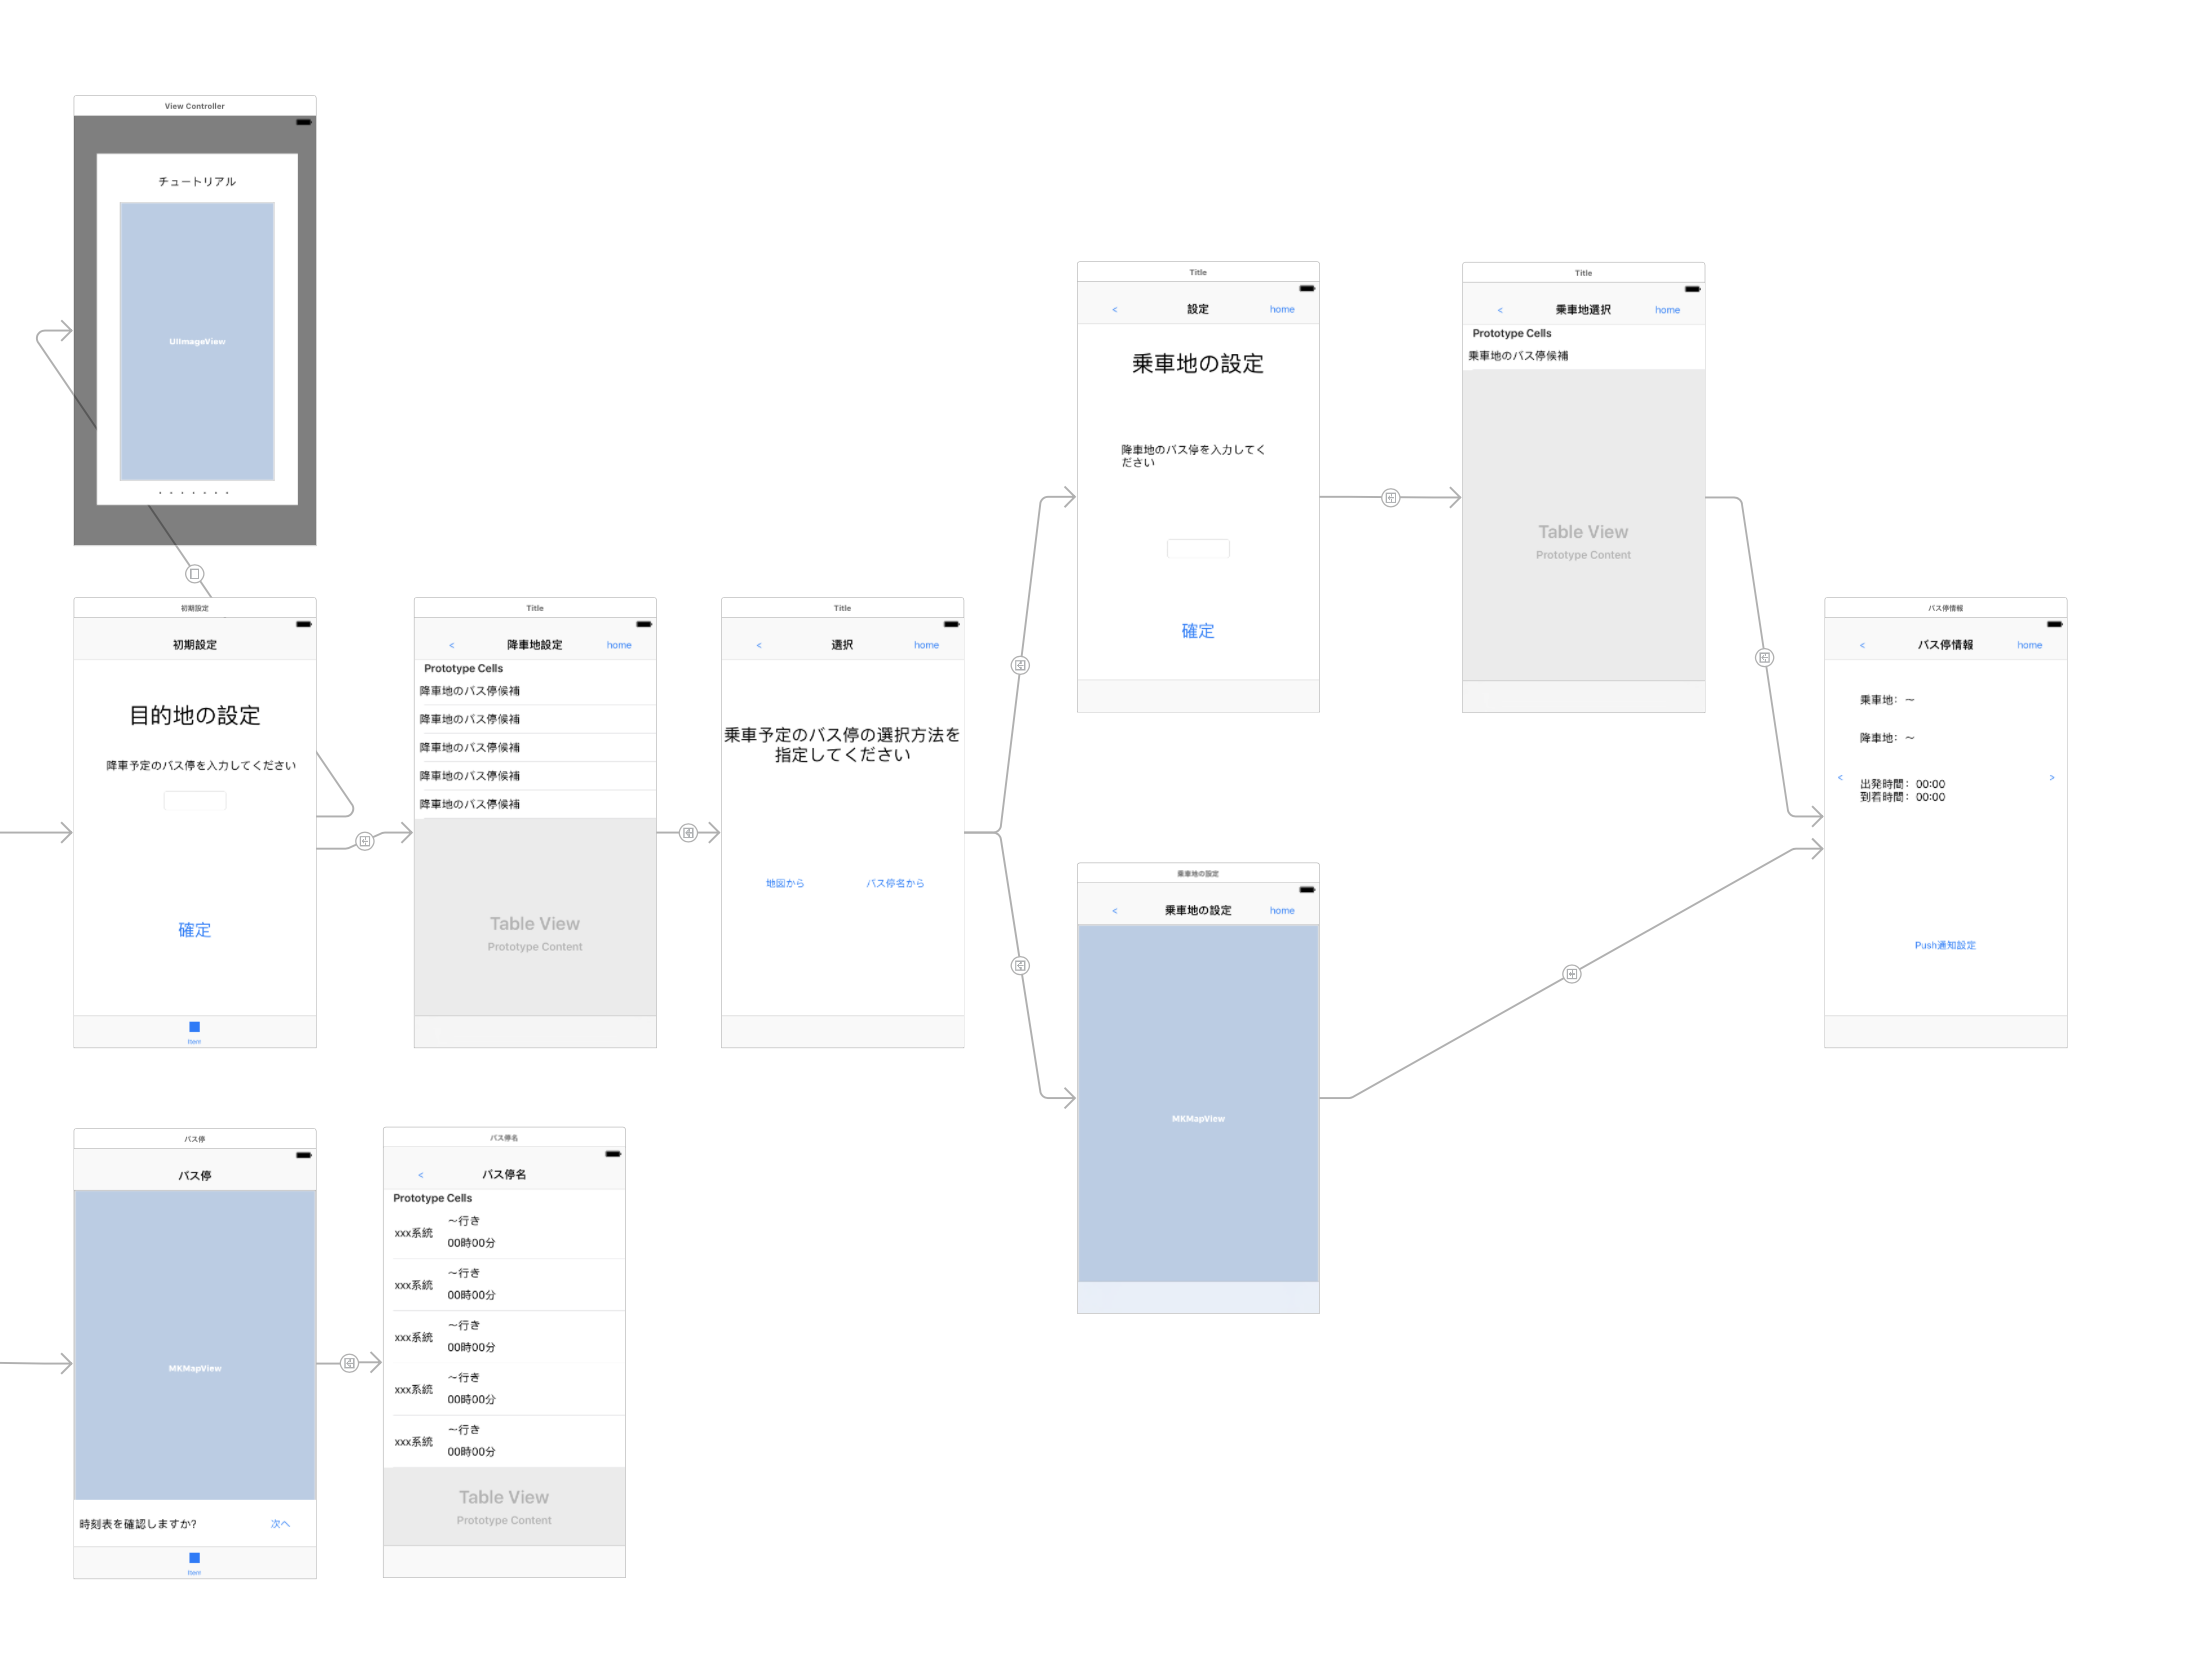
\includegraphics[clip,width=19cm,angle=90]{img/picture.png}
    \label{fig:senni}
  \end{center}
\end{figure}

\chapter{中間発表会ポスター}
\begin{figure}[htbp]
  \begin{center}
    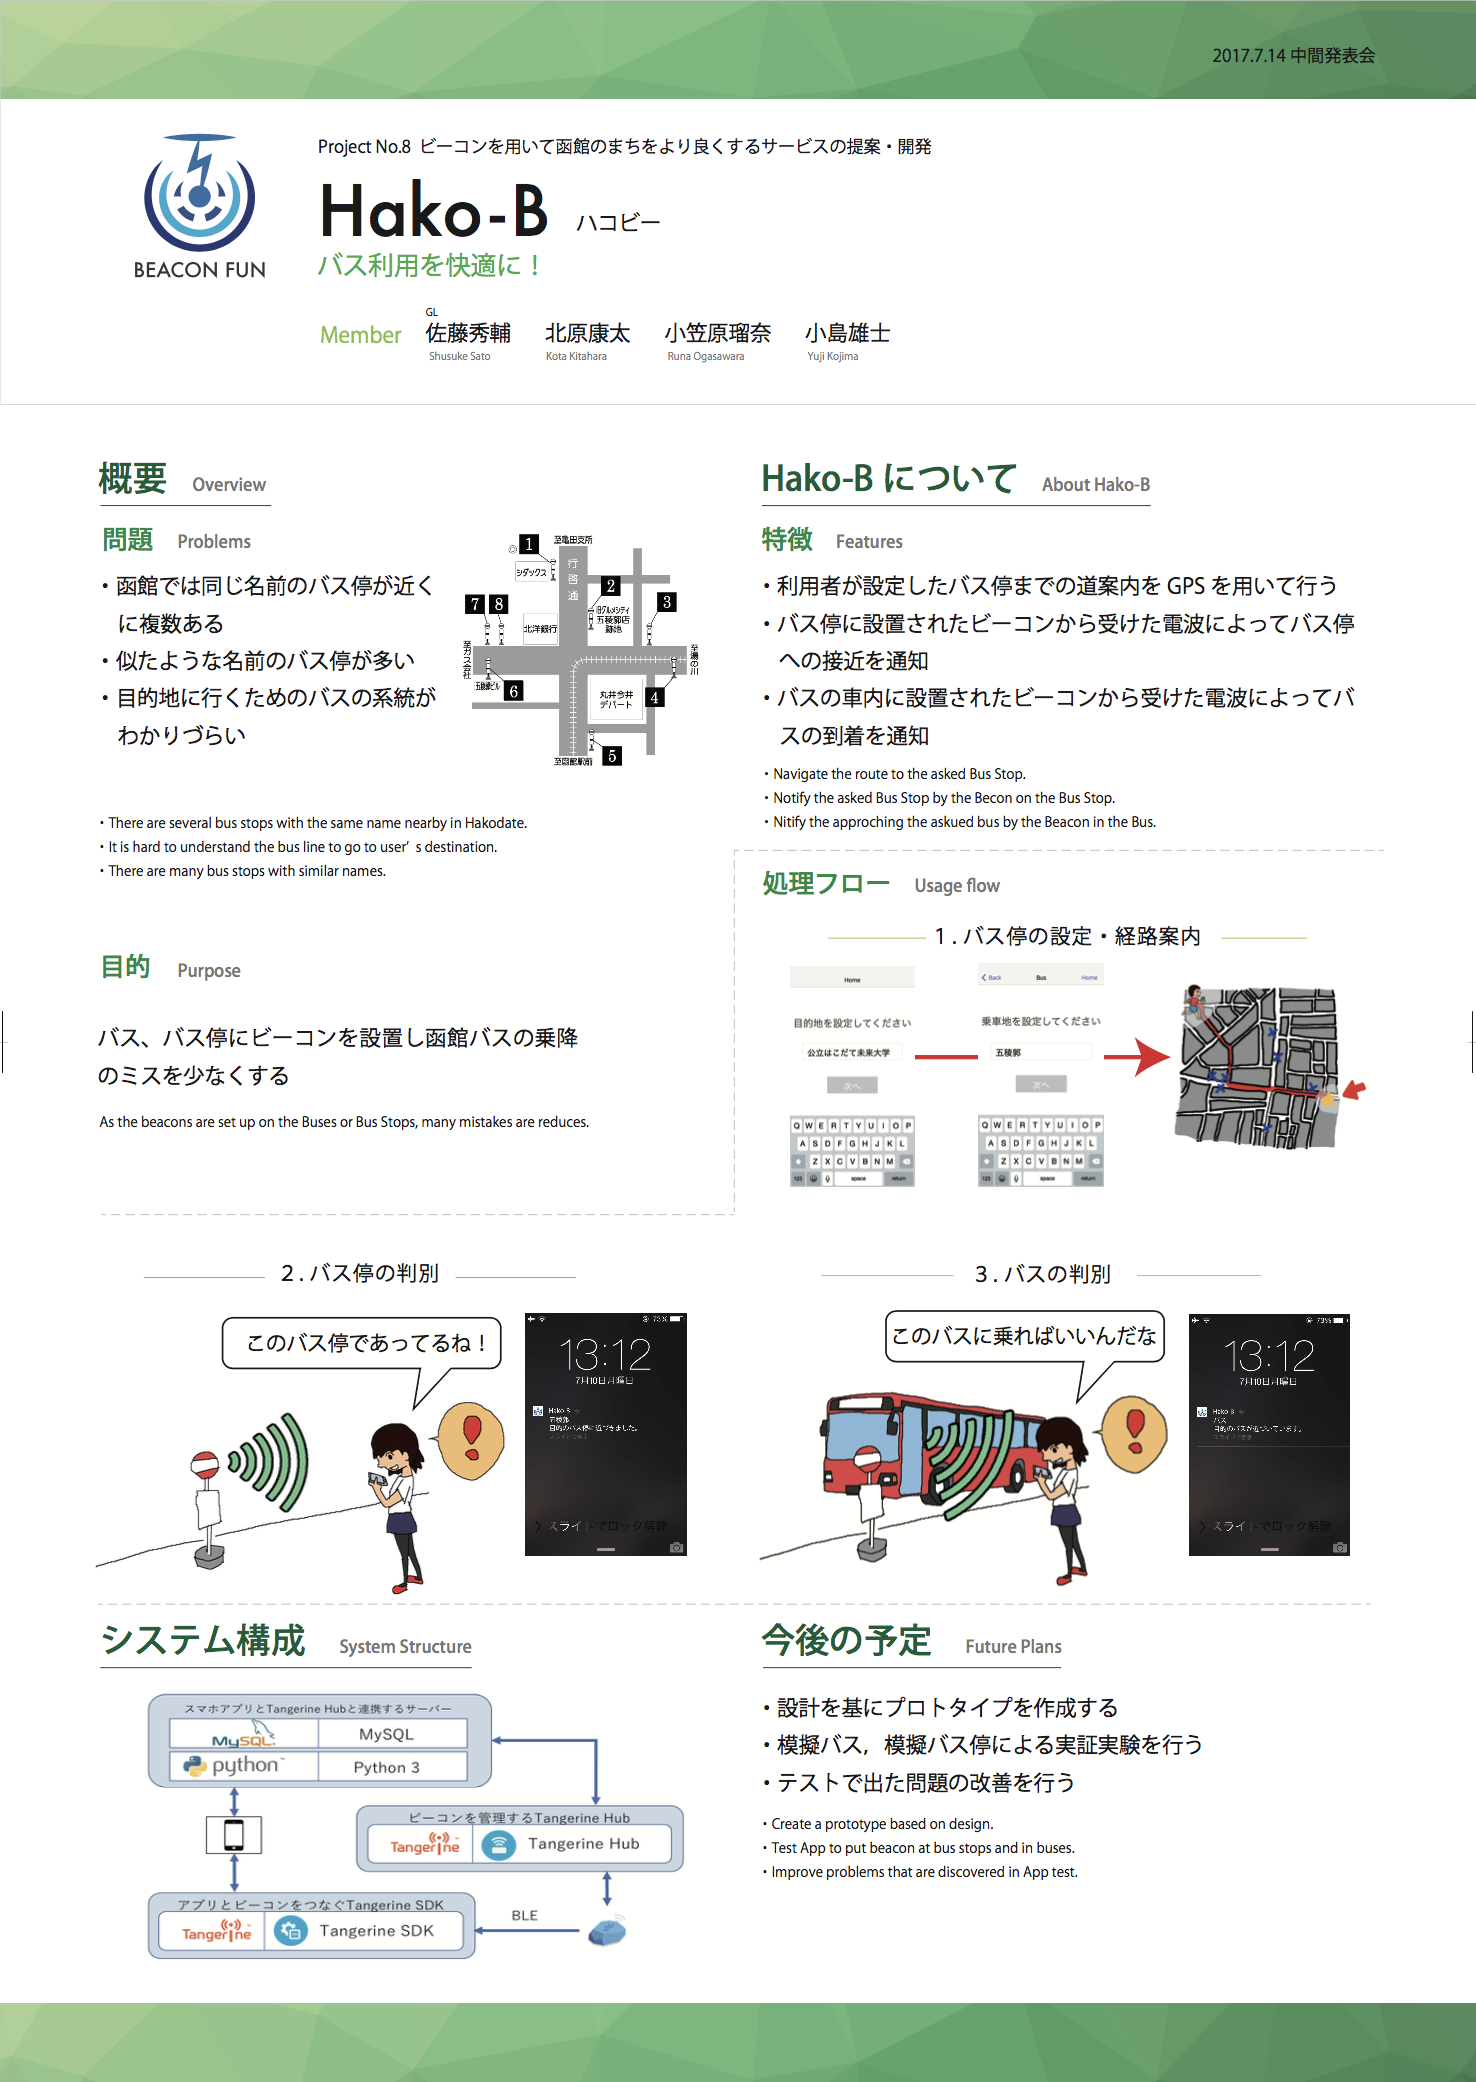
\includegraphics[clip,width=14cm]{img/poster.png}
    \label{fig:poster}
  \end{center}
\end{figure}

\chapter{成果報告会ポスター}
\begin{figure}[htbp]
  \begin{center}
    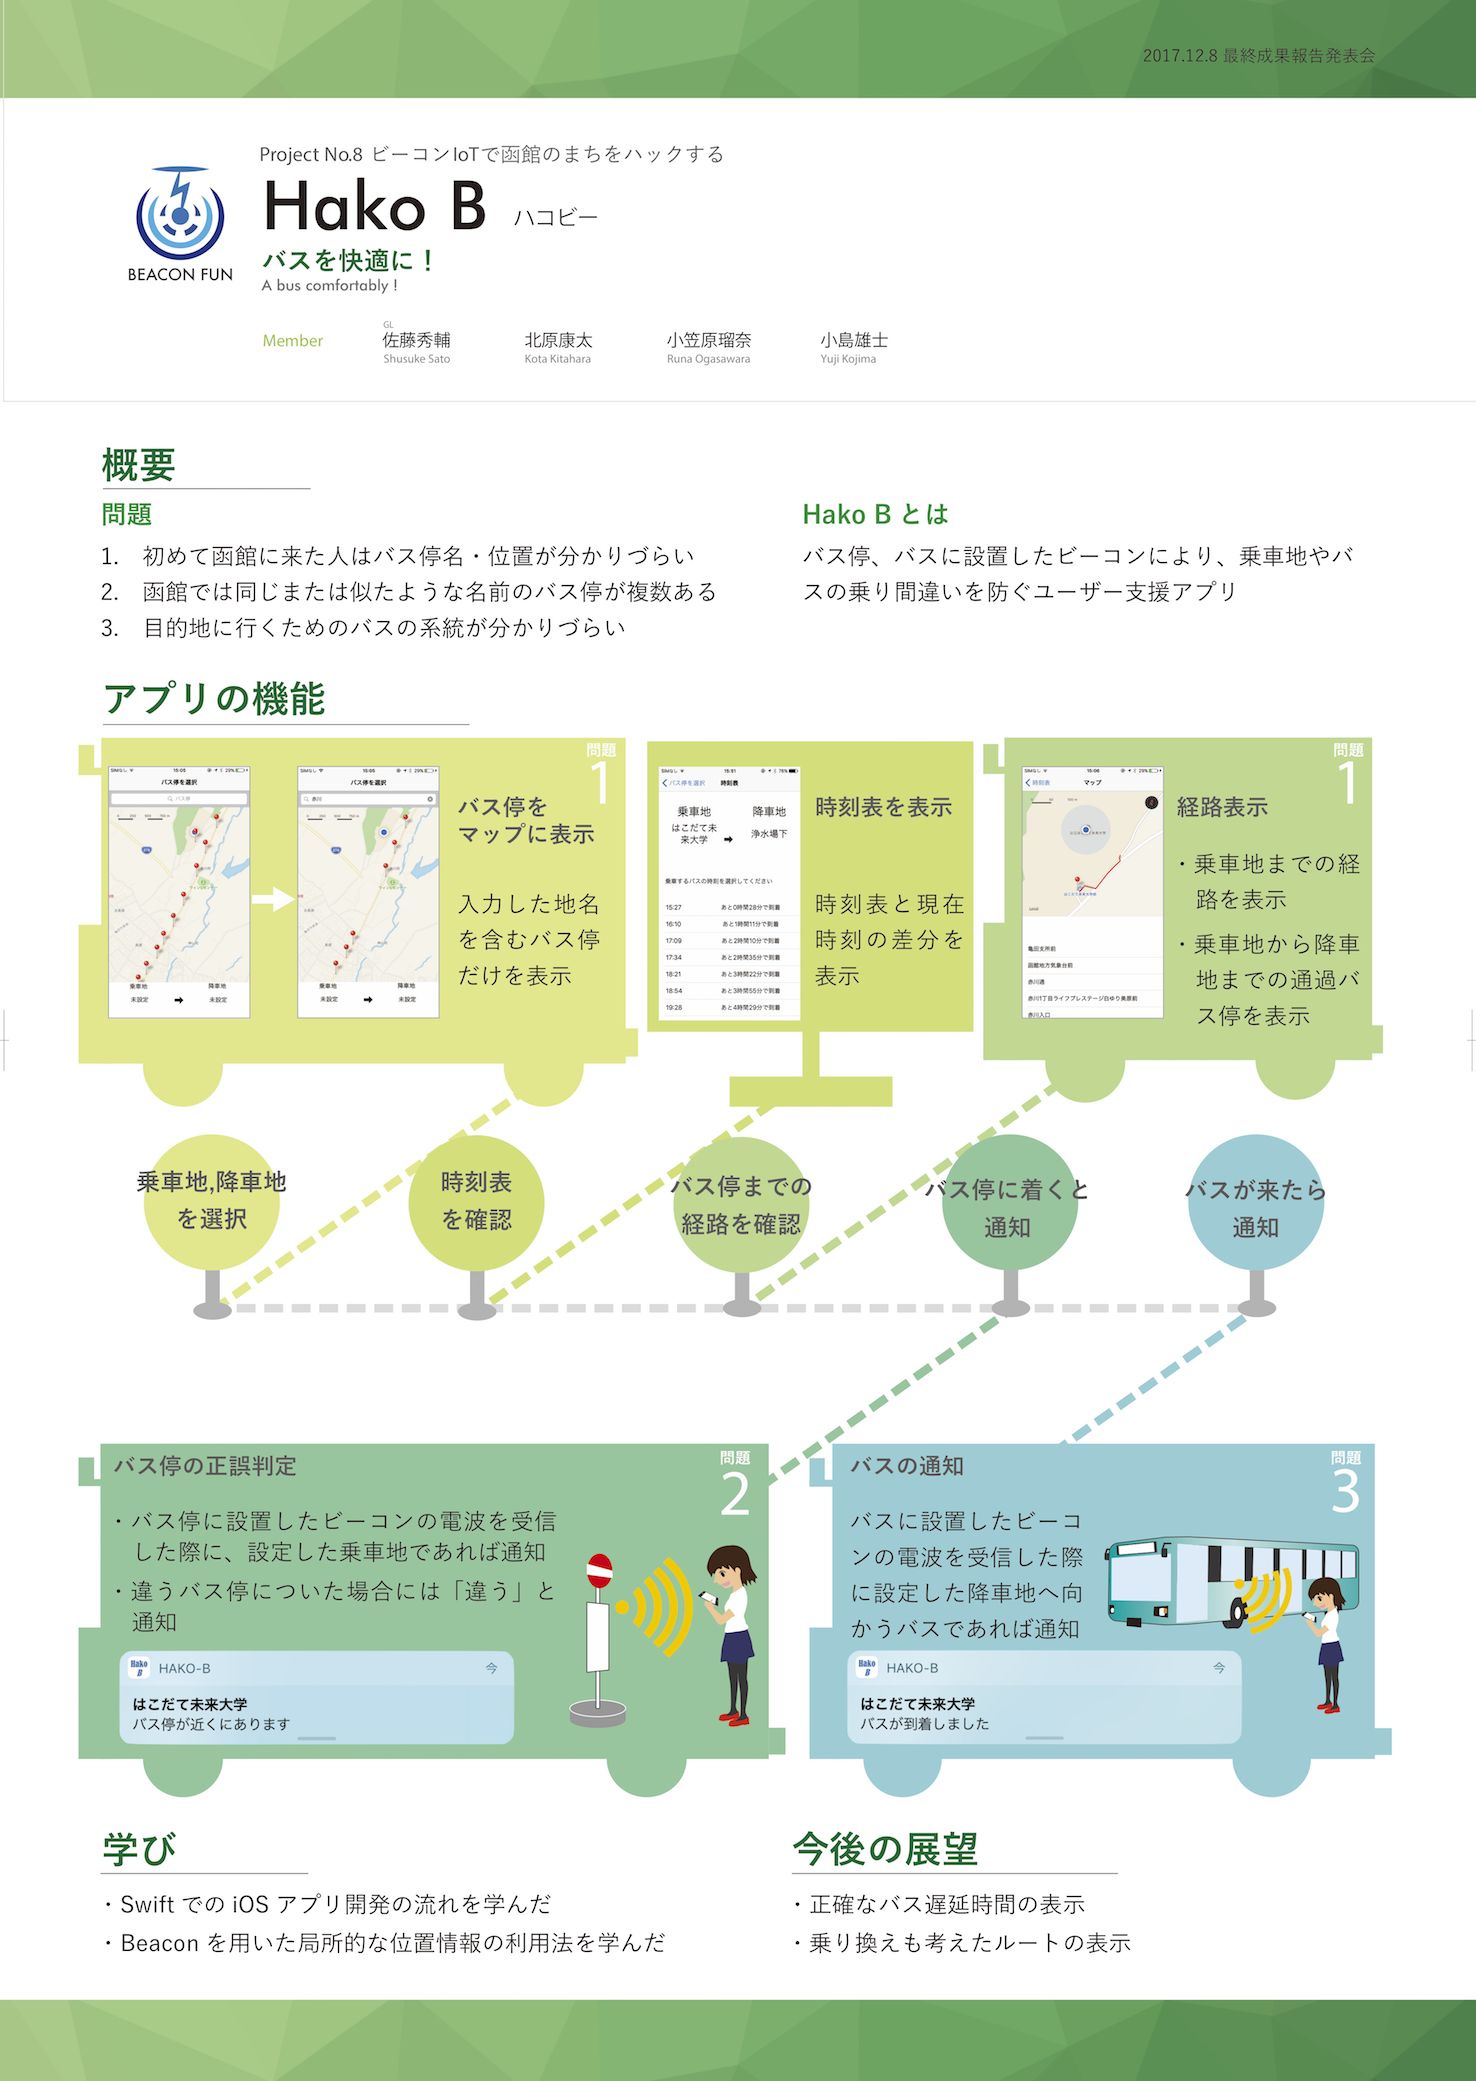
\includegraphics[clip,width=14cm]{img/final_poster.png}
    \label{fig:poster}
  \end{center}
\end{figure}
  
  %付録の終わり
  \end{appendix}
  
  
  %\backmatter

  \printbibliography[title=参考文献]
  
  \end{document}
  